\chapter{Hardware setup}\label{ch:hardware}
In order to connect to the camera and robot, a personal workstation has been used. Most of the time spent by our group was in the Robotics laboratory, where we worked and tested the ADEPT Cobra robot. We have placed inside the robot cell the camera needed to aquire images of the blocks for further processing. 

The phisical connections to the workstation were made through: 
\begin{itemize}
	\item Ethernet to the robot  
	\item USB to the camera 
\end{itemize}

\begin{figure}[hb]
\centering
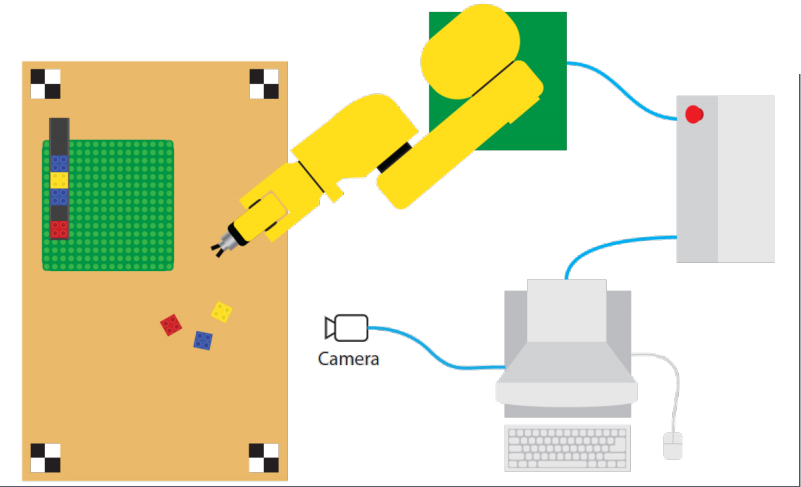
\includegraphics[width=4in]{figures/robotCellDesign.png}
\caption[robot Cell Design]
{A illustration of the robot Cell Design}
\end{figure}

The robot runs with the ADEPT Desktop program which is running on a local computer with Windows XP. This computer is connected to a switch nearby and has a static IP. Thus, we connect our workstation to that switch through a Ethernet cable and set a static IP on that port in order to connect to the ADEPT Desktop and using Matlab we send commands to the robot. Regarding the camera, it was needed to install the webcam package provided by Matlab in order to connect and properly use it. 
